\section{Fremstilling af speckle pattern} \label{Fremstilling af Speckle pattern}
Påføring af et speckle pattern i makroskala på en 2D flade, gøres på nuværende tidspunkt primært med enten spraydåse eller stempler. Det kan også gøres ved andre metoder såsom tusch eller midlertidige tatoveringer \parencite{Dong2017ACorrelation, Quino2021SpeckleEndurance}. Tidligere beskrevet i afsnit \ref{DIC afsnit}, afgrænses projektet til at skulle fremstille prikker i makroskala på $\geq \SI{0,1}{mm}$. Ved fremstilling af speckle pattern til DIC, ønskes det at parametrene er optimale, som beskrevet i afsnit \ref{Optimale speckle patterns}. 


\subsubsection{Spraydåser og Airbrush} \plainbreak{-.4}
Spraydåser og airbrushes producerer speckle patterns ved brug af trykluft til at blæse maling ud på en overflade. Spraymetoder er gode til at dække et område hurtigt og forholdsvist tilfældigt, idet malingens position kun kan bestemmes ved at ændre afstand til emnet, og retning som malingen udsendes i. Dette betyder, at malingen kan samles i større klumper, eller blive for sig selv i små pletter, der skaber unikke mønstrer, med stor variation i prikstørrelser. Dette kan være en udfordring, fordi der kan skabes for store mørke områder, eller kan ændre overfladetykkelsen. Derudover er airbrush og spraydåser begrænsede i, hvor store prikmønstrer de kan skabe. Dette overkommes ved at modificere på afstanden mellem emnet og dysen, dysens diameter, tryk i dysen og tykkelsen af væsken.\parencite{Dong2017ACorrelation, Quino2021SpeckleEndurance} 

Spraydåsen og airbrushen er ikke ens, og der er fordele ved, at bruge airbrush frem for spraydåser. Forskellen mellem airbrush og spraydåse kan ses på figur \ref{Spraymetode}, hvor de to billeder til venstre (a,b) er lavet med airbrush, og de to til højre (c,d) er udført med spraydåse. Her giver airbrushen et mere udspredt speckle pattern, og en større variation i prikstørrelse, som øger muligheden for unikke mønstre. Spraydåsen giver dog større risiko for afvigelse i prikstørrelserne, så der altid vil være prikker, der enten er for store eller for små til det ønskede speckle pattern. \parencite{Crammond2013SpeckleCorrelation}

\begin{figure}[H]
    \centering
    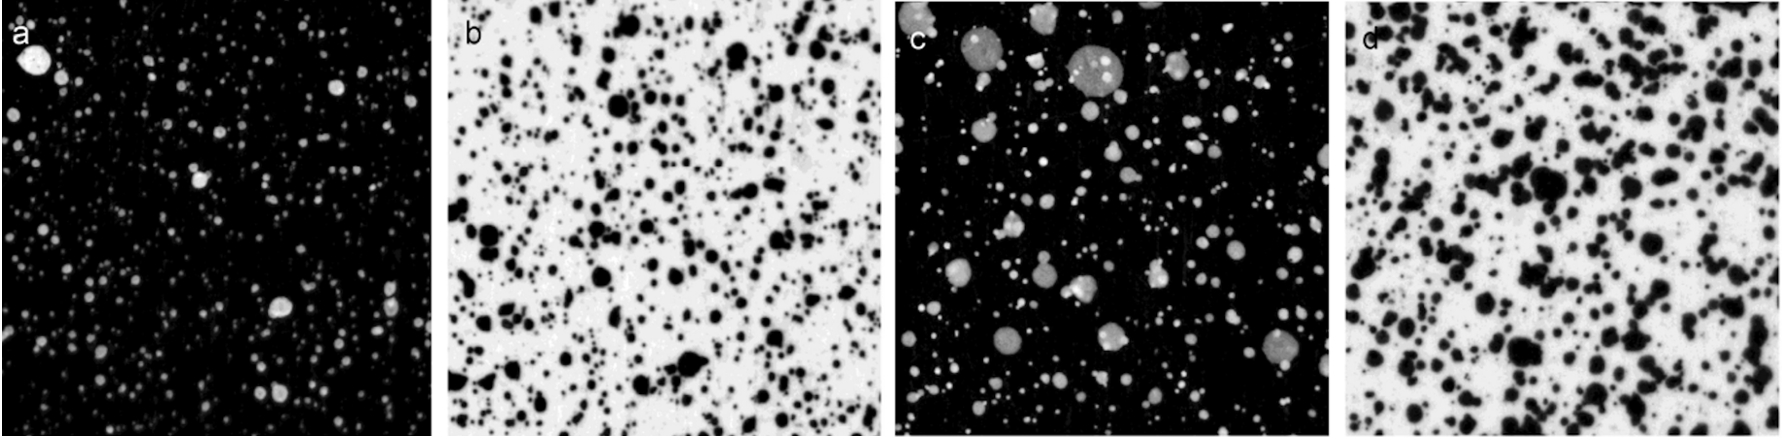
\includegraphics[width=1.0\linewidth]{Sections/2 Problemanalyse/Media/AirvsSprayinline.png}
    \caption{Speckle patterns med Airbrush og spraydåse. Her er a og b med Airbrush og c og d med Spraydåse \parencite{Crammond2013SpeckleCorrelation}}
    \label{Spraymetode}
\end{figure} \plainbreak{-0.5}


Spraydåsen er en priseffektiv metode til at påføre et  speckle pattern, hvor en spraydåse med 400 mL maling kan købes for 39,95kr. i Harald Nyborg (17.3.2025) \parencite{HaraldNyborg2025ColorWorksMat}. En airbrush har flere specialdele og kræver en kompressor for at virke, med det resultat, at den koster mere og anskaffe, modsat spraydåser \parencite{Dong2017ACorrelation}. Et airbrushsæt kan købes fra Amazon til omkring 600kr \parencite{TIMBERTECH2025Amazon.comAirbrush}.



\subsubsection{Stempel og stempelrulle} \plainbreak{-0.4}
Stemplet og stempelrullen er simple værktøjer til fremstilling af speckle pattern, da de ikke kræver andet end blæk at benytte. Anskaffelsesprisen er højere for stempelruller end airbrushes og spraydåser, hvor et sæt med 6 stempler, 6 ruller og noget blæk koster 2350\$ ($\simeq$ 16700 DKK, d. (25.2.2025)) hos Correlated Solutions. Eksempel på en stempelrulle kan ses i figur \ref{fig: Stempelrulle}. De størrelser der kommer i sættet fra Correlated Solutions, har stempelruller med prikdiametre fra $\SI{0,18}{mm}$ til $\SI{5,08}{mm}$, hvilket ved 1920:1080 opløsning, vil give en FOV fra $\SI{4,3}{cm}$ til $\SI{325}{cm}$. \parencite{CorrelatedSolutions2025VICCorrelation}

Stempler og rullerne virker ved, at blæk påføres deres overflade, som efterfølgende rulles over overfladen på emnet, hvor blækket overføres og efterlader et speckle pattern. Hvert stempel skaber mønstrer i en bestemt størrelse, hvilket begrænser antallet af forskellige emner og FOV'er det enkelt stempel kan bruges på, for at ramme 5-8 pixels pr. prik, som defineret i afsnit \ref{Speckle pattern}. \parencite{Dong2017ACorrelation}



\begin{figure}[H]
    \centering
    \begin{subfigure}{0.46\textwidth}
        \centering
        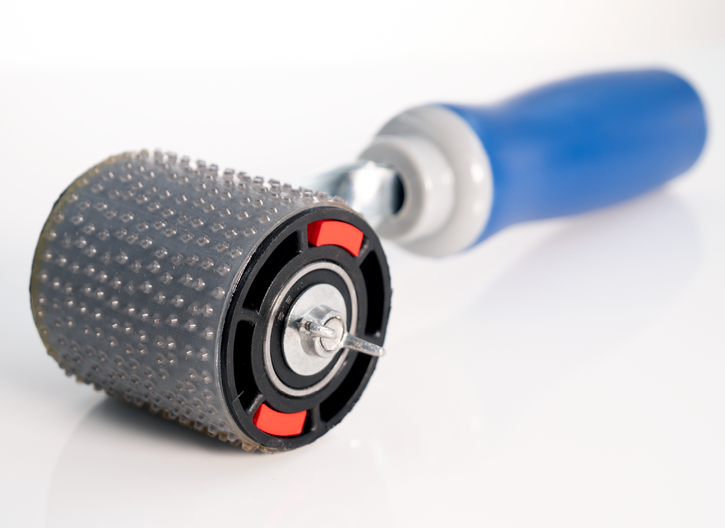
\includegraphics[width=.98\linewidth]{Sections/2 Problemanalyse/Media/Roller.png}
        \caption{Stempelrulle (\cite{CorrelatedSolutions2025VICCorrelation})}
        \label{fig: Stempelrulle}
    \end{subfigure}
    \begin{subfigure}{0.49\textwidth}
        \centering
         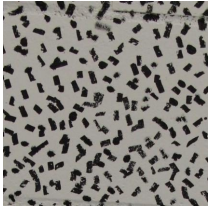
\includegraphics[width=0.7\linewidth]{Sections/2 Problemanalyse/Media/Tusch.png}
         \caption{Speckle pattern med overstregningstusch og lav densitet \parencite{HoseinSalmanpour2013PDFWalls}}
        \label{SpeckleTusch}
    \end{subfigure}
    \caption{}
    \label{fig:rulle og tush}
\end{figure} \plainbreak{-0.5}


\subsubsection{Tusch og andre skriveredskaber}  \plainbreak{-0.4}
En anden metode til påføring af speckle pattern, er tuscher og andre skriveredskaber, der sikre at prikkerne forbliver på overfladen af emnet under deformation. Et sæt med fire tuscher med en diameter på mellem \(\SI{0,1}{mm}\) og \(\SI{0,7}{mm}\) koster 13\$ ($\simeq$ 90 DKK, d. (6.3.2025)) \parencite{STAEDTLER2025Amazon.comTousch}. Metoden kræver, at prikkerne sættes manuelt én efter én på overfladen. Denne metode er tidskrævende, og kan være vanskeligt at opnå optimale parametre med, hvilket kan medføre fejlmålinger ved DIC, grundet mangel på nøjagtighed, som beskrevet i afsnit \ref{Speckle pattern}. Fordelen ved at prikkerne placeres manuelt er, at mønsteret ikke bliver isotropt. 
Det er et problem at prikkernes afstand mellem hinanden kan variere, da der kan skabes pletter, der er for store, eller områder med for lidt dækning af prikker, så der ikke kan observeres en deformation i de områder. Et eksempel på et speckle pattern tegnet med overstregningstusch kan ses i figur \ref{SpeckleTusch} \parencite{HoseinSalmanpour2013PDFWalls}. Usikkerheden ved metoden kan mindskes, hvis tiden der bruges på at sætte prikkerne øges. 





%Det er muligt at finde specielle tuscher eller kuglepenne, der er lavet med meget små spidser, så der kan laves prikker med en diameter på 100$\mu m$, som kan bruges i FOV'er helt ned til 2,2cm på langs (med en opløsning på 1920:1080).\parencite{Dong2017ACorrelation}.  her kan det blive et problem, da usikkerhederne kan medføre at der kommer klatter af ren farve eller andre fejl såsom mere farve end 70\% eller mindre end 50\%, som kan medføre fejlmålinger i DIC, grundet mangel på præcision (\ref{Speckle pattern}). Dette er muligt at undgå, hvis der bruges endnu længere tid på at gøre sine prikpositioner perfekte, som medfører mere tid brugt ved mindre skala.


\subsubsection{Midlertidig tatovering}  \plainbreak{-0.4}
En midlertidig tatovering, bruges til at overføre et bestemt mønster over på en flade. Dette fungerer ved, at der genereres et speckle pattern, som laserprintes ind på tatoveringspapiret. Herefter kan tatoveringen klistres på den ønskede overflade, hvorefter den vædes, så blækket overføres og forbliver på overfladen. Prisen på to A4 ark printbart papir til midlertidige tatoveringer koster 9.99\$ ($\simeq$ 69 DKK, d. 17.3.25) \parencite{SilhouetteAmerica2025TemporaryClearMEDIA-TATTOO-3T}. Det kræver en laserprinter, for at kunne printe en midlertidig tatovering, hvilket øger anskaffelsesprisen for denne metode.\parencite{Quino2021SpeckleEndurance}

\begin{comment}
    \begin{figure}[H]
    \centering
    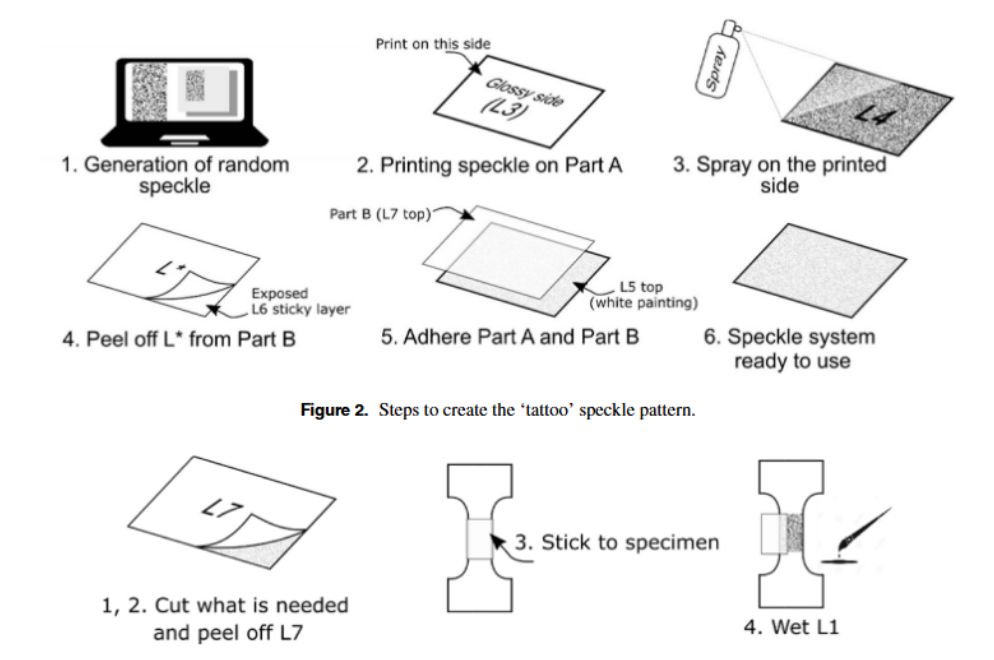
\includegraphics[width=0.8\linewidth]{Sections/2 Problemanalyse/Media/Temporary tattoo.png}
    \caption{Fremgangsmåde ved påføre af midlertidig tatovering med speckle pattern \parencite{Quino2021SpeckleEndurance}}
    \label{Midlertidigtatovering}
\end{figure}
\end{comment}



\subsection{Robotter til fremstilling af speckle pattern}  \label{Robotter til fremstilling af speckle pattern}
De nuværende produkter på markedet, der benyttes til fremstilling af speckle pattern, kræver manuelt arbejde og har varierende nøjagtighed i densitet og størrelse af prikker. På baggrund heraf vurderes det, at brugen af robotter til fremstilling af speckle patterns kan automatisere processen og har potentiale for at øge genskabeligheden. Sådan en løsning muliggør altå at der kan laves mere ensartetede prøver af flere af samme emnetype og dermed øges nøjagtigheden af DIC.


%Den mest brugte metode er spraydåsen, altså spraydåser og airbrush \parencite{Dong2017ACorrelation, Quino2021SpeckleEndurance}. Det vil altså være optimalt at kunne lave en løsning, der er mere effektiv end denne løsning. Spraymetoden er optimeret i forhold til pris og påføringshastighed, hvor spraydåser er engangsforbrug, og airbrush kan genbruges, men kræver en kompressor og maling. Det er derfor svært at slå disse to i pris og påføringshastighed, og det er derfor et ønske at lave et bedre produkt, som er bedre til at danne speckle patterns end spraymetoden er.

%En af de ting som spraymetoden ikke er god til, er at den er lidt for tilfældig, og store mængder maling kan samle sig på samme sted. Det vil derfor være et ønske, at løsningen skal kunne skabe et præcist mønster pålideligt, hvilket indebærer at der ikke skabes prikker mindre end 3 og større end 7 pixels (\ref{Speckle pattern}).

